\chapter{C}
\section{Hello World}
\begin{code}[ht!]
	\inputminted[linenos]{c}{codes/helloWorld.c}
	\caption{Hello World in C}
\end{code}

\begin{remark}
	Need to compile using a compiler like \mintinline{bash}{clang} or
	\mintinline{bash}{gcc}.
\end{remark}

\section{Input}
\begin{code}[ht!]
	\inputminted[linenos]{c}{codes/helloUser.c}
	\caption{Hello User in C}
\end{code}

\begin{remark}
	In case of errors in compiling, start by trying to \emph{fix} the first one, and so on.
\end{remark}

\begin{remark}
	Use \mintinline{bash}{-lcs50} to link \mintinline{c}{cs50.h} header.
\end{remark}

\begin{remark}
	Use \mintinline{bash}{make} to ease your life compiling!
\end{remark}

\clearpage
\section{Initialization}
\begin{minted}{c}
	int counter = 0;
\end{minted}

\section{Increment}
\begin{minted}{c}
	counter = counter + 1;
	counter += 1;
	counter++; // Syntactic Sugar
\end{minted}

\section{Conditionals}
\begin{minted}{c}
	if (x < y)
	{
		printf("x is less than y!\n");
	}
	else if (x > y)
	{
		printf("x is greater than y!\n");
	}
	else // if (x == y)
	{
		printf("x is equal to y!\n");
	}
\end{minted}

\section{Loops}
\subsection{While Loop}
\subsubsection{Infinite Loop}
\begin{minted}{c}
	while(true)
	{

	}
\end{minted}

\subsubsection{Repeat}
\begin{minted}{c}
	int i = 0;
	while(i < 50)
	{
		printf("Hello World!\n");
		i = i+1;
	}
\end{minted}

\subsection{For Loop}
\begin{minted}{c}
	for(int i = 0; i < 50; i += 1)
	{
		printf("Hello World!\n");
	}
\end{minted}

\section{Additional Info}
\subsection{Datatypes}
Some of these (like \mintinline{c}{string}) are implemented in \mintinline{c}{cs50.h} library.
\begin{itemize}
	\item \mintinline{c}{bool}
	\item \mintinline{c}{char}
	\item \mintinline{c}{double}
	\item \mintinline{c}{float}
	\item \mintinline{c}{int}
	\item \mintinline{c}{long}
	\item \mintinline{c}{string}
	\item \dots
\end{itemize}

\subsection{Functions}
They are implemented in \mintinline{c}{cs50.h} library.
\begin{itemize}
	\item \mintinline{c}{get_char}
	\item \mintinline{c}{get_float}
	\item \mintinline{c}{get_double}
	\item \mintinline{c}{get_int}
	\item \mintinline{c}{get_long}
	\item \mintinline{c}{get_string}
	\item \dots
\end{itemize}

\subsection{Placeholders}
\begin{itemize}
	\item \mintinline{c}{%c} for \mintinline{c}{char}
	\item \mintinline{c}{%f} for \mintinline{c}{float}
	\item \mintinline{c}{%i} for \mintinline{c}{int}
	\item \mintinline{c}{%li} for \mintinline{c}{long}
	\item \mintinline{c}
\end{itemize}


\section{Examples}
\subsection{Arithmetic}
\begin{code}[ht!]
	\inputminted[linenos]{c}{codes/int.c}
	\caption{int.c}
\end{code}

\begin{code}[ht!]
	\inputminted[linenos]{c}{codes/float.c}
	\caption{float.c}
\end{code}

\begin{code}[ht!]
	\inputminted[linenos]{c}{codes/parity.c}
	\caption{parity.c}
\end{code}

\clearpage
\subsection{Conditional}
\begin{code}[ht!]
	\inputminted[linenos]{c}{codes/conditions.c}
	\caption{conditions.c}
\end{code}

\clearpage
\subsection{Logical}
\begin{code}[ht!]
	\inputminted[linenos]{c}{codes/agree.c}
	\caption{agree.c}
\end{code}

\clearpage
\subsection{Loop}
\begin{code}[ht!]
	\inputminted[linenos]{c}{codes/src1/cough0.c}
	\caption{cough0.c}
\end{code}

\begin{code}[ht!]
	\inputminted[linenos]{c}{codes/src1/cough1.c}
	\caption{cough1.c}
\end{code}

\clearpage
\subsection{Function}
\begin{code}[ht!]
	\inputminted[linenos]{c}{codes/src1/cough2.c}
	\caption{cough2.c}
\end{code}

\begin{code}[ht!]
	\inputminted[linenos]{c}{codes/src1/cough3.c}
	\caption{cough3.c}
\end{code}

\begin{code}[ht!]
	\inputminted[linenos]{c}{codes/src1/positive.c}
	\caption{positive.c}
\end{code}

\begin{code}[ht!]
	\inputminted[linenos]{c}{codes/src1/mario0.c}
	\caption{mario0.c}
\end{code}

\begin{code}[ht!]
	\inputminted[linenos]{c}{codes/src1/mario2.c}
	\caption{mario2.c}
\end{code}

\begin{code}[ht!]
	\inputminted[linenos]{c}{codes/src1/mario8.c}
	\caption{mario8.c}
\end{code}

\clearpage
\section{Limitations}
\begin{code}[ht!]
	\inputminted[linenos]{c}{codes/src1/floats.c}
	\caption{floats.c}
\end{code}

\begin{code}[ht!]
	\inputminted[linenos]{c}{codes/src1/overflow.c}
	\caption{overflow.c}
\end{code}

\blfootnote{Click \href{pdfs/src1.pdf}{here} for more examples.}

% \clearpage
% \section{Source Code}
% Find some pre-compiled examples below
% 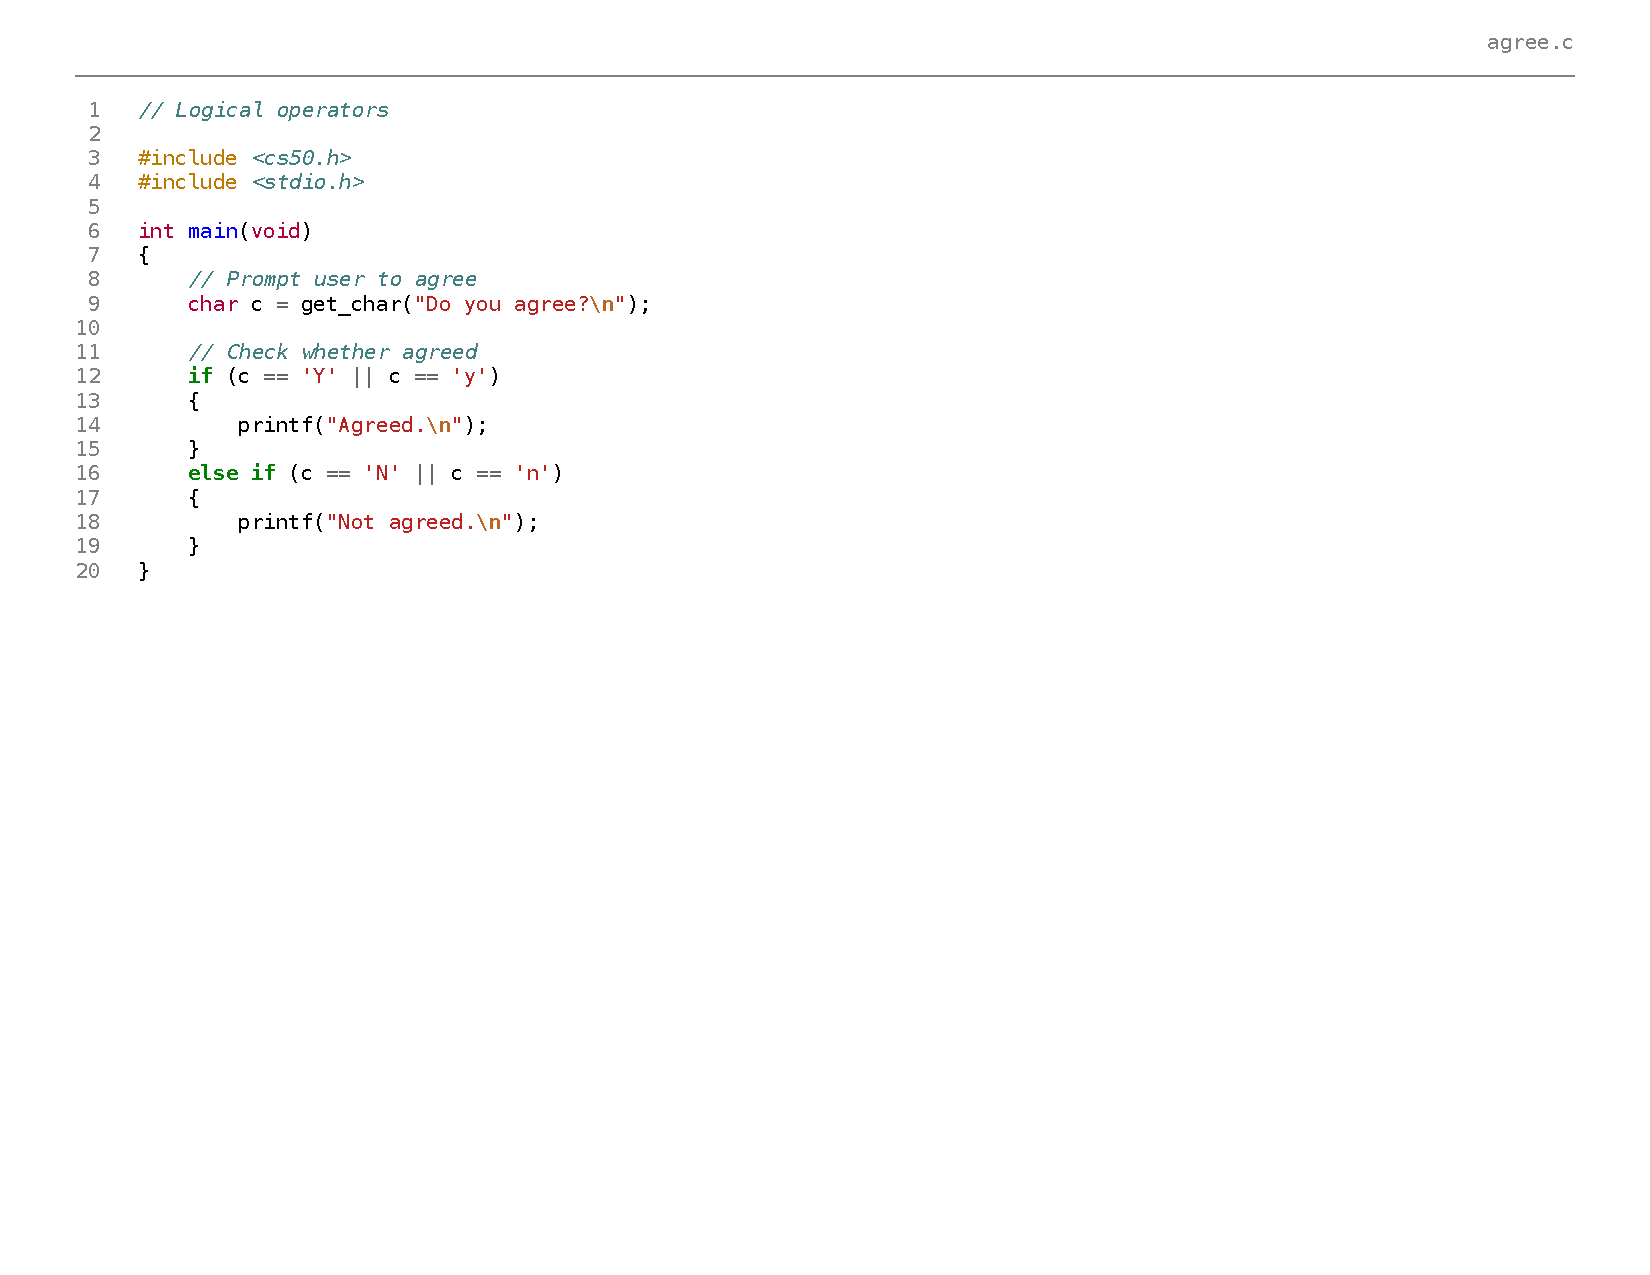
\includepdf[pages=-]{pdfs/src1.pdf}